\subsection{Законы Кеплера}
\paragraph{I-ый закон} Все планеты движутся по
эллиптическим орбитам, в одном из фокусов которых
находится Солнце.

Введём обозначение $u \equiv 1/r$, тогда момент импульса планеты можно найти, как
\begin{equation*}
	L = \sigma 2 m = m r^2 \omega = \frac{m}{u^2} \frac{d \theta}{d t},
\end{equation*}
где $\theta$~--- угловая координата в полярной системе координат, центр которой находится в центре Солнца.
Выразим $dt$ из полученного выражения для момента импульса планеты:
\begin{equation*}
	dt = \frac{m}{L u^2} \, d\theta.
\end{equation*}

Найдем теперь первую производную длины радиус-вектора по времени:
\begin{equation*}
	\frac{d r}{d t} = \frac{d}{d t} \left( \frac{1}{u} \right) = - \frac{1}{u^2} \frac{du}{dt},
\end{equation*}
подставим сюда выражение для $dt$:
\begin{equation*}
	\frac{d r}{d t} = - \frac{1}{u^2} \frac{du \cdot L u^2}{m \, d \theta} = - \frac{L}{m} \frac{d u}{d \theta}.
\end{equation*}

Далее получим выражение для второй производной:
\begin{equation*}
	\frac{d^2 r}{dt^2} = \frac{d}{dt} \left( - \frac{L}{m} \frac{d u}{d \theta} \right) = -\frac{L}{m} \frac{d^2 u}{dt \, d \theta},
\end{equation*}
аналогично проделанному ранее, подставим сюда выражение для $dt$.
\begin{equation*}
	\frac{d^2 r}{dt^2} = - \frac{L^2	 u^2}{m^2} \frac{d^2 u}{d \theta^2}.
\end{equation*}

Запишем теперь уравнение движения планеты в гравитационном поле Солнца~--- результирующая сила, действующая на планету равна сумме силы гравитационного притяжения и центробежной силы.
\begin{gather*}
	m \frac{d^2 r}{d t^2} = - \frac{G M m}{r^2} + m \omega^2 r,\\
	- \frac{L^2	 u^2}{m^2} \frac{d^2 u}{d \theta^2} = - GMu^2 + \frac{L^2}{r^4 m^2} \cdot r,\\
	\frac{d^2 u}{d \theta^2} + u = \frac{GM m^2}{L^2}.
\end{gather*}
Общее решение полученного неоднородного уравнение есть сумма общего решения однородного уравнения 
\begin{equation*}
	\frac{d^2 u}{d \theta^2} + u = 0
\end{equation*}
и частного решения неоднородного уравнения. В качестве частного решения возьмём 
\begin{equation*}
	u(\theta) = \frac{GM m^2}{L^2} = \const.
\end{equation*}
Однородное уравнения является уравнением гармонических колебаний, поэтому его решение можно представить в виде
\begin{equation*}
	u(\theta) = A \cos \theta,	
\end{equation*}
где $A$~--- постоянная интегрирования, определяемая из начальных условий. Отсюда общее решение неоднородного уравнения запишется, как
\begin{equation*}
	u(\theta) = \frac{GM m^2}{L^2} + A \cos \theta \equiv \frac{1}{r(\theta)}.
\end{equation*}

В качестве начальных условий рассмотрим такие: $r(0) = s$, $L = m\sqrt{G M h}$, где $s$ и $h$ пока только некоторые расстояния. Подставив выбранные начальные условия в решение уравнения, получим, что
\begin{gather*}
%	\frac{1}{s} = \frac{GM m^2}{m^2 G M h} + A,\\
	A = \frac{s - h}{sh}.
\end{gather*}
В итоге решение уравнение примет вид
\begin{gather*}
	\frac{1}{r} = \frac{1}{h} + \frac{s - h}{sh} \cos \theta,\\
	r = \frac{sh}{s + (s - h) \cos \theta},\\
	r = \frac{h}{1 + \dfrac{s - h}{s} \cos \theta}.
\end{gather*}

Получили уравнение эллипса в полярных координатах, где $(s - h)/s$~--- эксцентриситет $e$, $h$~--- фокальный параметр $p$, а $\theta$~--- истинная аномалия $\nu$. Это завершает доказательство первого закона Кеплера. Для задачи двух тел доказательство аналогично, если воспользоваться \imp{приведённой массой}.

\paragraph{II-ой закон} Радиус-вектор планеты за
равные промежутки времени заметает равные площади:
\begin{equation}
	\frac{dS}{dt}=\const = \frac{S_\text{элл}}{T} = \frac{\pi a b }{T}.
\end{equation}


\paragraph{III-ий закон} Квадраты периодов обращения планет
относятся как кубы больших полуосей их орбит.
\begin{equation}
	\frac{T^2_1}{T^2_2}=\frac{a^3_1}{a^3_2},
\end{equation}
где $a$ --- большая полуось, $T$ --- период обращения.
\begin{figure}[h!]
	\begin{minipage}[b]{0.5\textwidth}
		\centering
		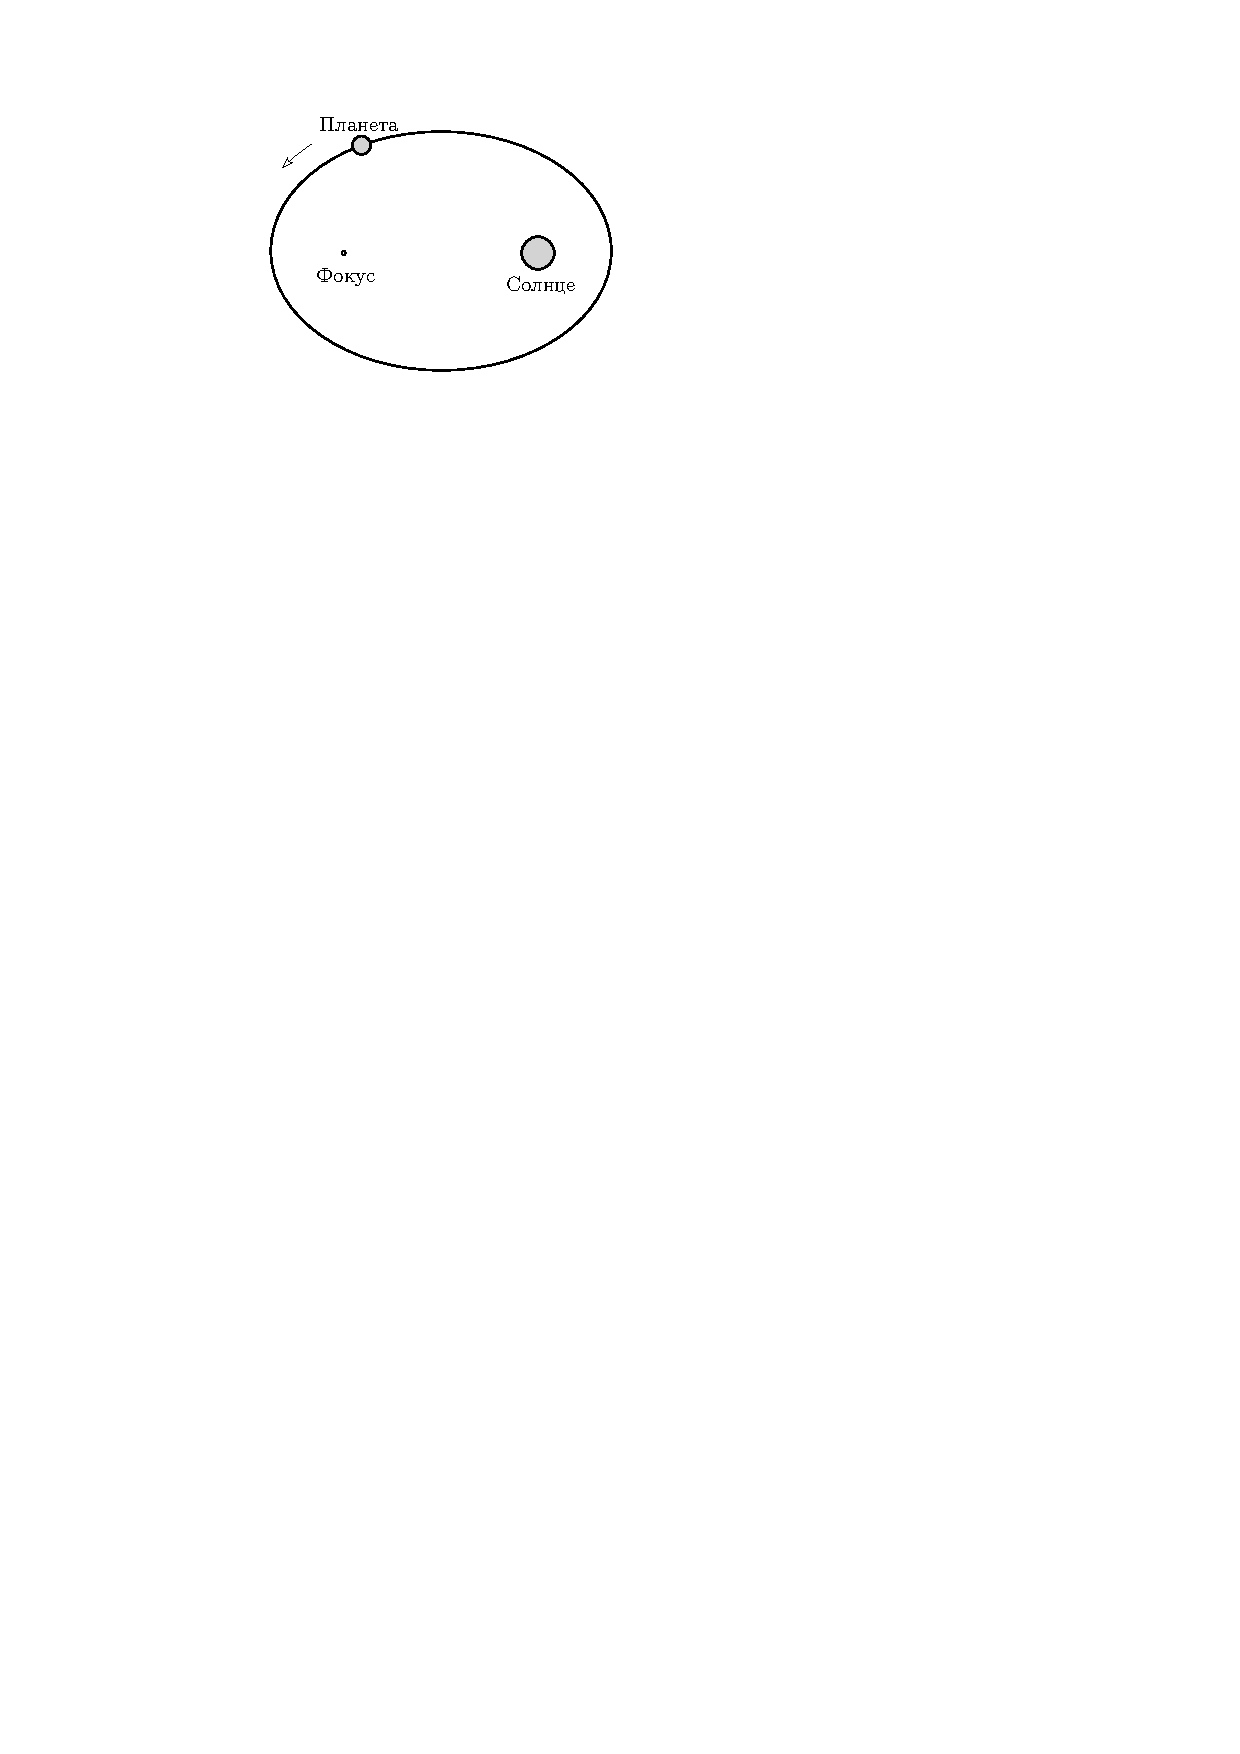
\includegraphics[width = 0.84\textwidth]{first-kepler}
		\caption{Первый закон Кеплера}
	\end{minipage}
	\begin{minipage}[b]{0.5\textwidth}
		\centering
		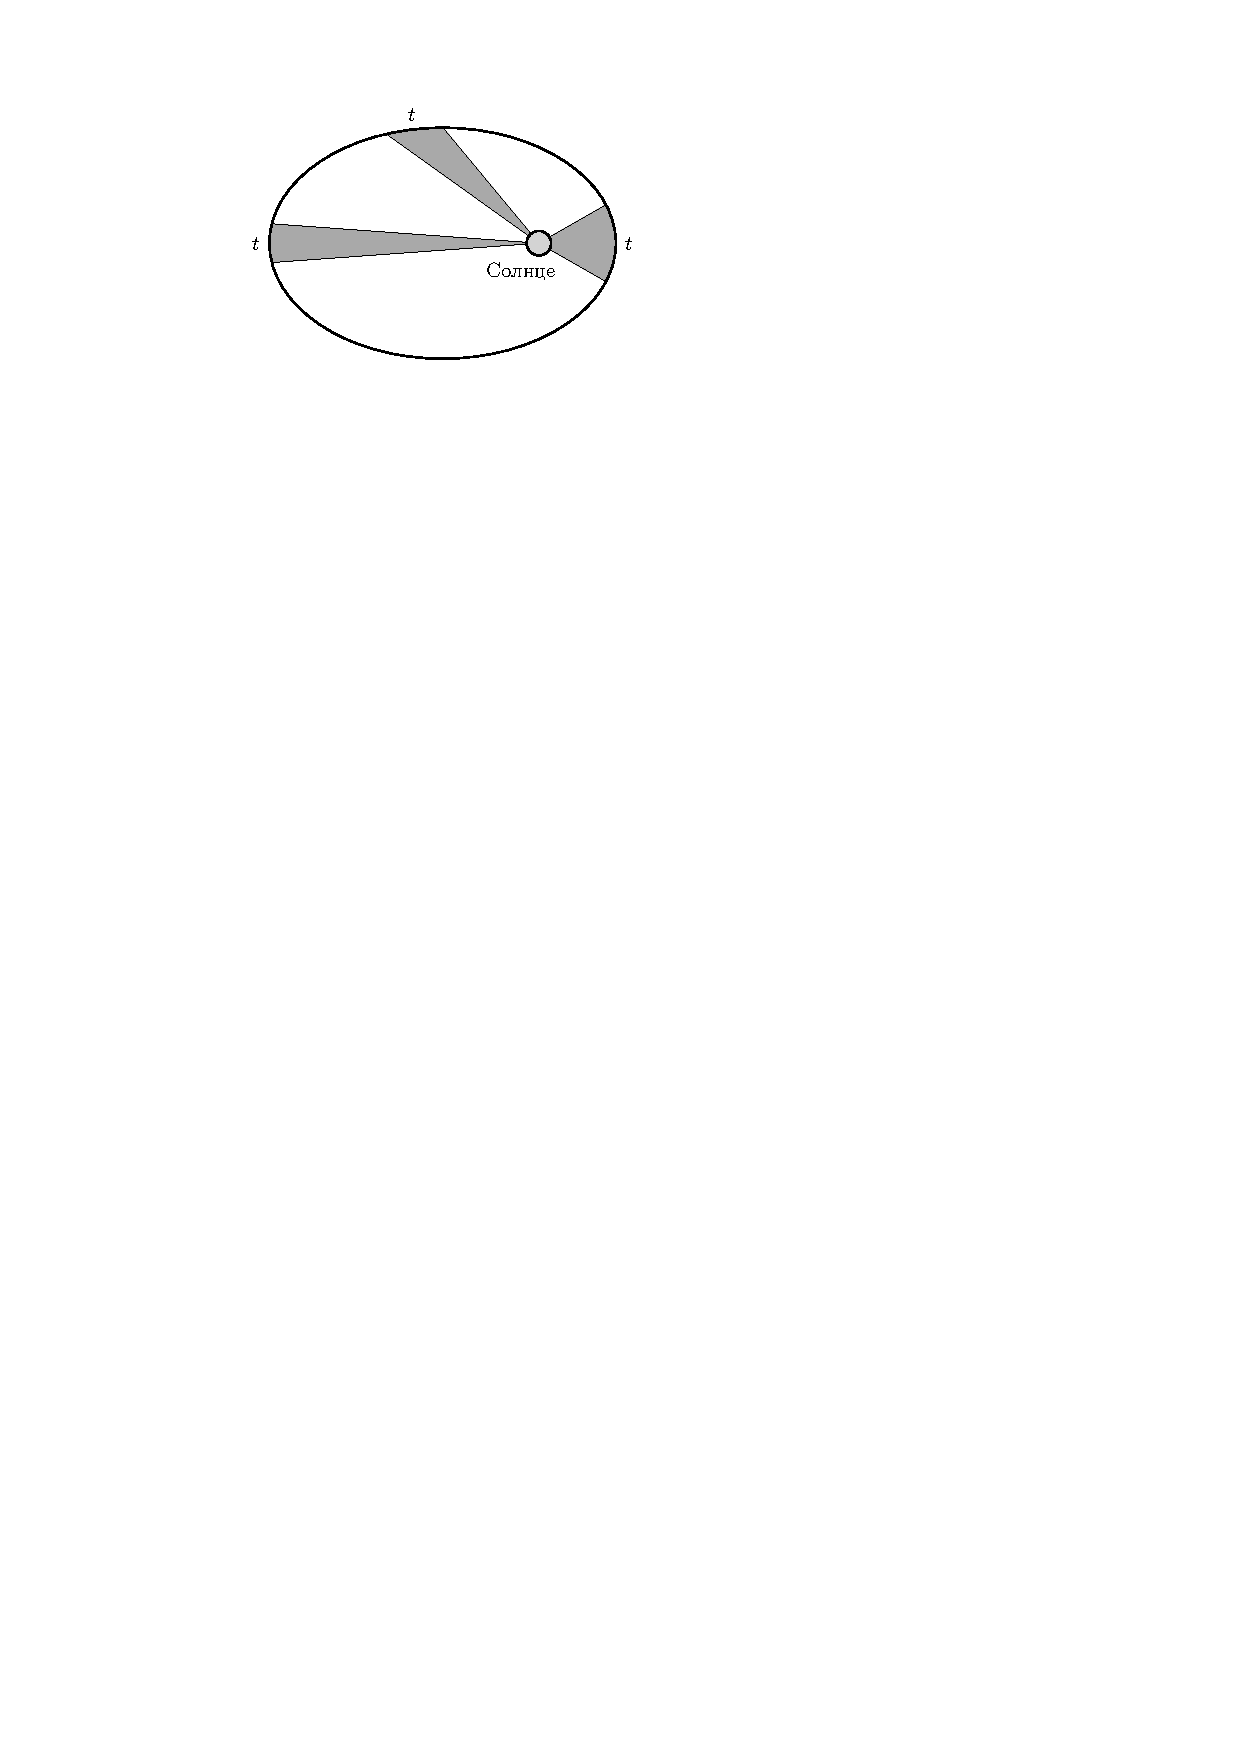
\includegraphics[width = 0.972\textwidth]{second-kepler}
		\caption {Второй закон Кеплера}
	\end{minipage}
\end{figure}

Получим \imp{третий закон Кеплера}, заметив, что модуль секториальной скорости можно записать, как
\begin{gather*}
	\sigma
	= \frac{S_\text{эл}}{T}
	= \frac{\pi a b}{T}
	= \frac{L}{2m},\\
	\frac{\pi a^2 \sqrt{1 - e^2}}{T}
	= \frac{m \sqrt{\dfrac{GM}{a} \cdot \dfrac{1 + e}{1 - e}} \cdot a(1-e)}{2m},\\
	\frac{4\pi^2 a^4 (1 - e^2)}{T^2}
	= a^2(1-e)^2 \cdot \frac{GM}{a} \cdot \frac{1 + e}{1-e}
\end{gather*}
\begin{equation}
	\frac{T^2}{a^3} = \frac{4\pi^2}{GM}.
\end{equation}

\term{Обобщённый} Ньютоном \term{III-ий закон Кеплера} имеет следующий вид:
\begin{equation}
	\frac{T^2_1( M_1 + m_1)}{T^2_2( M_2 + m_2 )}=\frac{a^3_1}{a^3_2} \quad \Longleftrightarrow \quad
	\frac{T^2 ( M + m )}{a^3} = \frac{4 \pi^2}{G},
\end{equation}
где $M_1$ и $M_2$~--- массы центральных тел, $m_1$ и
$m_2$~--- массы обращающихся вокруг них тел. Так как массы планет
$m$ много меньше массы звезды $M$, $M + m \simeq M$.
